\section{Approach}

Algorithm \ref{algo:core-exp} summarizes the main steps of our approach.
In this section we present these steps in detail and give an end-to-end example.
We build an area with a high density of points, decide where to place it on the grid,
and then build the rest of the solution around it.
Human experts are known to sometimes take such a strategy as well.

As seen in the pseudocode, our approach takes as input a \emph{pattern} $p$, besides
the thematic dictionary and the regular dictionary.
A {pattern} is a rectangular grid of a given size, with zero or more black cells and no letters.

\begin{figure}
\centering
\begin{tabular}{ccc}
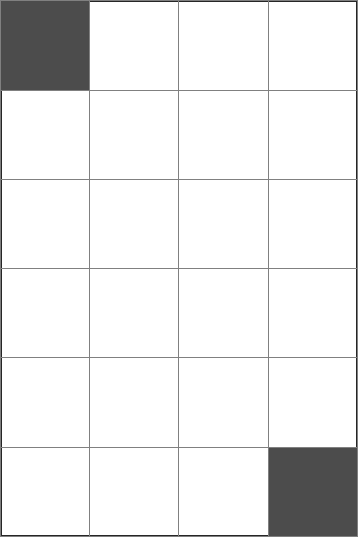
\includegraphics[width=.15\textwidth]{_plots/6x4-puzzle.pdf} & &
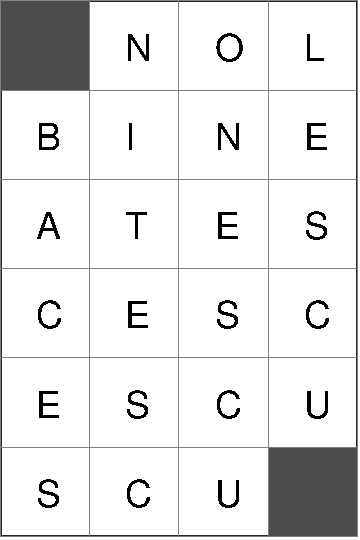
\includegraphics[width=.15\textwidth]{_plots/core-6x4-puzzle.pdf}
\end{tabular}
\caption{Left: A pattern defined as a $6 \times 4$ grid with two black cells, in the top-left corner and the bottom-right corner. Right: A core based on the pattern at hand.}
\label{fig:pattern}
\end{figure}

Figure \ref{fig:pattern} (left) shows an example of a pattern. It is a $6 \times 4$ grid with two black cells, one in the top-left corner and one in the bottom-right corner.
Observe that the pattern is significantly smaller than the $13 \times 13$ size of the full-size grid.
The pattern will end up being integrated inside the full-size solutions generated with our approach
as we will show in this section.

\begin{algorithm}[t]
\DontPrintSemicolon % Some LaTeX compilers require you to use \dontprintsemicolon instead
\KwIn{Pattern $p$, thematic dictionary and regular dictionary}
%\KwOut{Full solutions}
%\tcc{Search for a full solution}
$C \leftarrow \mbox{GenerateCores}(p)$\; \label{algl:generateCores}
$E \leftarrow \mbox{ExpandCores}(C)$\; \label{algl:expandCores}
$S \leftarrow \mbox{GenerateSeeds}(E)$\; \label{algl:generateSeeds}
Rank $S$ and put top $k$ elements into a list $S'$\; \label{algl:rankSeeds}
\For{$s \in S'$} {
    $\mbox{Evolve}(s)$\; \label{algl:evolveSeeds}
}
\caption{{\sc Generating full solutions.}}
\label{algo:core-exp}
\end{algorithm}


\subsection{Generating Cores}

Step 1 in Algorithm \ref{algo:core-exp} generates a collection of so-called \emph{cores} from the pattern $p$.
A core is a pattern filled with letters on the white cells.
Figure \ref{fig:pattern} (right) shows an example of a core.

We require that in a full solution returned by Algorithm~\ref{algo:core-exp}, 
the sub-area corresponding to the pattern will have a perfect score.
That is each white cell in the pattern must contribute two points.\vb{reworded}

To achieve this we construct a small crosswords puzzle instance
and solve it with 
{\sc Wombat},
a freely available C++  solver for crosswords optimization.
{\sc Wombat} takes as input up to two dictionaries (one thematic and one regular),
and a grid with the black cells in place, and zero or more letters.
The program is very effective at computing high scores when such input 
is provided, including all black cells~\cite{DBLP:conf/socs/BoteaB21,Botea_Bulitko_2022}. \vb{added ``all black cells''}

In the small instance we build,
the grid is the pattern $p$. There is only one dictionary, which contains 
substrings of the thematic words.\footnote{No regular dictionary is
needed here, as we seek a perfect score for this instance.}
It is sufficient to consider only substrings of the lengths that 
correspond to the lengths of the word slots in the pattern.

In our running example, the lengths of the pattern word slots are 3, 4, 5 and 6.
For example, when generating substrings of length 4,
if {\sf\small IONESCU} and {\sf\small POPESCU} are thematic words,
the substrings generated are {\sf\small IONE}, {\sf\small ONES}, {\sf\small NESC}, {\sf\small ESCU}, {\sf\small POPE}, {\sf\small OPES}, {\sf\small PESC} and {\sf\small ESCU}.
Duplicates such as {\sf\small ESCU} are kept only once.

We then run {\sc Wombat} to enumerate all solutions to the small instance, which are precisely the 
cores computed at step 1 in Algorithm \ref{algo:core-exp}.\vb{Changed ``set'' to ``run''. Should we mention that it is possible to run Wombat to find {\em all} solutions instead of just one?}



\subsection{Expanding Cores}

\begin{figure}
\centering
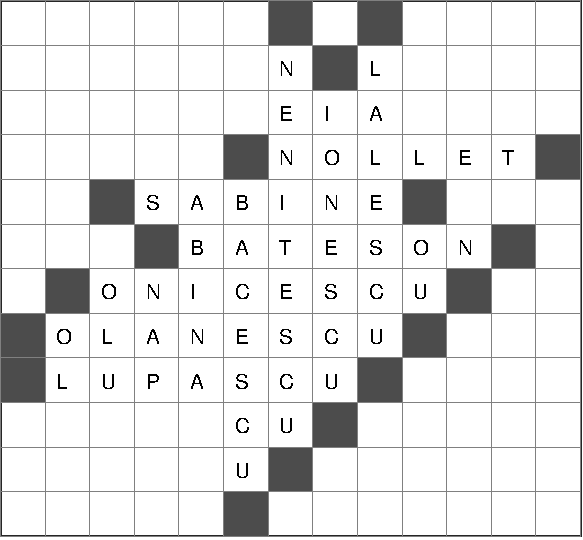
\includegraphics[width=.45\textwidth]{_plots/extcore-alive-0-puzzle-72-2975-1488--1--1.pdf}
\caption{An expanded core based on the core shown in Figure \ref{fig:pattern} (right).}
\label{fig:exp-core}
\end{figure}


At step 2 each core is expanded by placing full thematic words on top of the substrings present in the core at hand.
For each thematic word added to an expanded core, we add two black cells at its corresponding endpoints.
Figure \ref{fig:exp-core} shows an example of an expanded core. 
The cells on the top row, bottom row, leftmost column and rightmost column form the \emph{border} of the expanded core. The rest of the cells are the \emph{inner part} of the expanded core.
We define the \emph{inner size} as $h \times w$, where $h$ is the number of rows
of the inner part and $w$ is the number of columns.
In Figure \ref{fig:exp-core}, the inner size is $10 \times 11$.
Observe that the border can only contain black cells and empty cells.
The inner part can contain letters, black cells and empty cells.

As shown later in this section, the inner part of an extended core will be fit inside a full solution.
All or part of the border may or may not be included in a full solution, as explained later on.

More than one expanded core can exist for a given core (e.g., a substring such as {\sf\small ESCU} can be expanded into multiple thematic words such as {\sf\small IONESCU} and {\sf\small POPESCU}).
We generate expanded cores with a depth-first search.

We say that an extended core is a deadend (or, equivalently, it is dead) if no full valid solution can contain the extended core at hand. We label an extended core as dead, and filter it away, if any of the
following conditions is met:
it contains a word repetition; it contains a sequence of letters that cannot
possibly be expanded into a full word; or it contains adjacent black cells within the inner part.
Note that, at this stage, we do not check for adjacent black cells on the border.
Such a test will be performed later, after it is decided which part of the
border, if any, will be kept in a full-size solution. We detail this later in this section.\vb{reworded}


\subsection{Generating Seeds}

\begin{figure*}
\centering
\begin{tabular}{ccc}
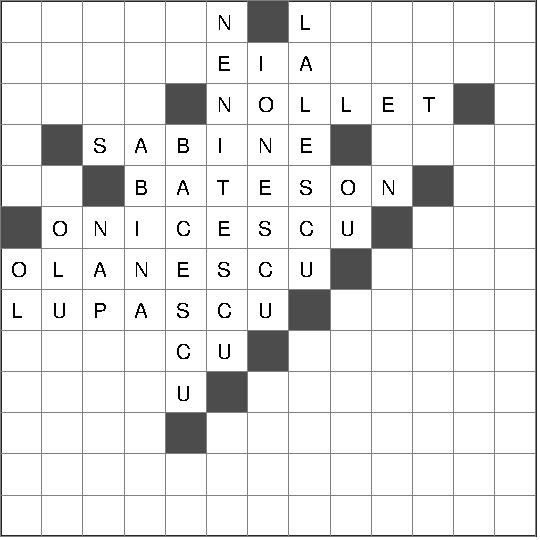
\includegraphics[width=.32\textwidth]{_plots/alive-0-puzzle-72-2975-1488--1--1.pdf} &
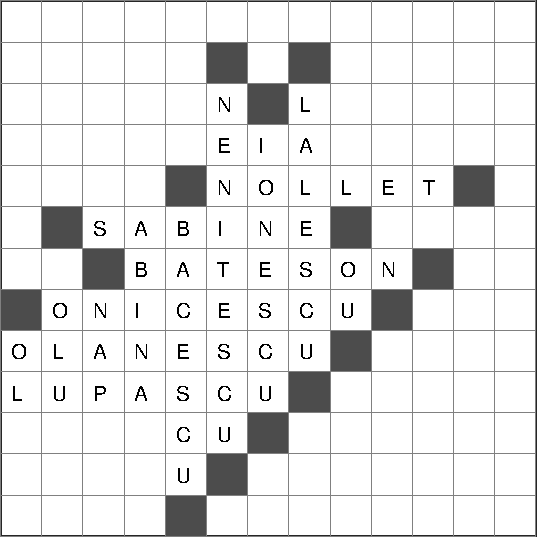
\includegraphics[width=.32\textwidth]{_plots/alive-0-puzzle-72-2975-1488--1-1.pdf} & 
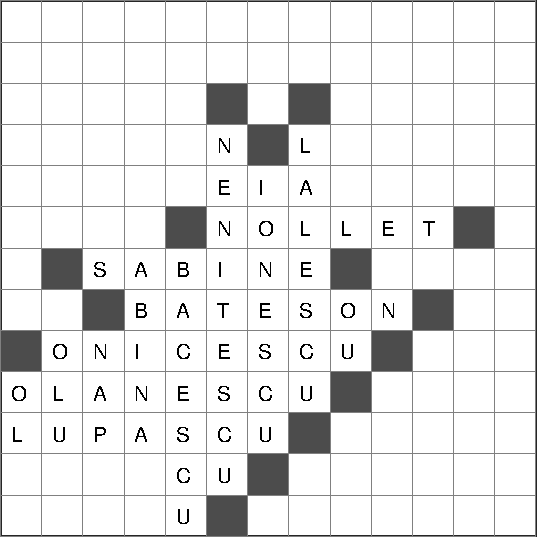
\includegraphics[width=.32\textwidth]{_plots/alive-0-puzzle-72-2975-1488--1-2.pdf}
\end{tabular}
\caption{Seeds generated from the extended core shown in Figure \ref{fig:exp-core}.}
\label{fig:seeds}
\end{figure*}

When the inner size of an extended core $e$ is $13 \times 13$, it fits inside a full $13 \times 13$ grid in a unique way. However,
if the inner height and/or width are below $13$, $e$ can fit inside a full grid in multiple positions,
obtained by shifting it inside the full grid vertically and/or horizontally.

Each fitting of an extended seed inside a full grid is called a \emph{seed}.
As such, a seed is a full-size $13 \times 13$ grid, with 
letters, black cells and empty cells.
Figure \ref{fig:seeds} shows three seeds generated from an extended core.

When the first column of the inner part of $e$ coincides 
with the first column of the seed, the leftmost column of $e$'s border
is left out from the seed. 
Otherwise, it is kept within the seed.
Other parts of the border (top row, bottom row, rightmost column)
are left out or kept inside in a similar way.
For example, in Figure \ref{fig:seeds} (left), the leftmost border column 
and the top border row are left out.
The seed in Figure \ref{fig:seeds} (middle) leaves out the
leftmost border column.
The seed at the right of Figure \ref{fig:seeds} leaves out
the leftmost border column and the bottom border row.


A seed is post processed with two objectives: to detect, if possible, dead seeds 
(e.g., seeds that cannot be possibly expanded into a valid full solution); 
and, for seeds that are still alive, to detect, if possible, 
forced black cells and forced letters that could be added to the seed.
Given a position (cell) in a seed,
we say that a black cell or a letter is forced onto a 
given position if 
every possible full solution based on that seed must contain 
the black cell or letter at hand on the corresponding position.

Algorithm \ref{algo:fixpoint} shows seed post-processing in pseudocode.
Deadend detection includes checking for closures and semi-closures;
adjacent black cells;\footnote{As this test is applied to the full
grid, it covers the part of the extended seed border, if any, that was
kept in the seed.}
word repetitions; and
sequences of letters that do not match with any word from the dictionaries.

Forced black cells are detected when all dictionary words matching 
a given sequence of letters in the seed would start in the same cell,
forcing the placement of a black cell on the cell before.
Similarly, forced black cells can be detected when 
all matching words finish on the same cell, forcing a black cell 
on the cell after.
Forced letters are detected when all matching words have the same 
letter on a given position, and it is not possible to insert
a black cell between the sequence of letters and the cell where
the forced letter is being added. 
This includes the case
where exactly one word matches the sequence of letters at hand,
forcing the addition of the entire word, and its corresponding
black cells to border the word.\footnote{No black cell needs to be added
at a given end of the forced word if the word 
is adjacent to the border of the grid at that endpoint.}

\begin{algorithm}[t]
\DontPrintSemicolon % Some LaTeX compilers require you to use \dontprintsemicolon instead
\KwIn{Seed $s$ labelled alive}
%\KwOut{Full solutions}
%\tcc{Search for a full solution}
\Repeat{reaching fixpoint} {
    \If {deadend detected} {
        Label $s$ as dead\;
        Break\;
    }
    Add forced moves (black cells and words) to $s$\;
}
\Return $s$ and label (dead/alive)
\caption{{\sc Fixpoint computation.}}
\label{algo:fixpoint}
\end{algorithm}

%%%%%%%%%%%%%%%%%%%%%%%%%%%%%%%%%%%%%%%%%%%%%%%%%%%%%%%%%%%%%%%%%%%%%%%%%%%%%%%%%%%%%%%%%%%%%%

\subsection{Ranking Seeds}
\label{sec:ranking}

Given a seed (i.e., a $13 \times 13$ grid with some letters and $n$ black cells) we need to complete it with an additional $26-n$ black cells\footnote{While having $26$ black cells is not a requirement for a legal crossword puzzle, having all allowed black cells ($26$ for a $13 \times 13$ grid) tends to maximize the score once the words are placed onto the grid.} 
so that {\sc Wombat} can 
subsequently attack the instance and fill the remaining white area with words.
The placement of the black cells should allow {\sc Wombat} to obtain a high score on the resulting instance.

There are two principally different ways of placing the remaining $26-n$ black cells: one-shot and incremental modifications. Indeed, one can place all $26-n$ black cells in one shot and then submit the resulting grid to {\sc Wombat} to fill in the words and compute the score. Alternatively, one can take an existing grid with $26$ black cells and move its black cells around (protecting the letters and black cells from the original seed) in an attempt to improve the score. A grid modified (or mutated) in such a way is then submitted to {\sc Wombat} again to compute its new score and the process repeats. One can view this process as an evolution of grids with {\sc Wombat} being the (slow) fitness function.

The first way of completing a seed to a full grid is faster since {\sc Wombat} is invoked only once. The second way is slower but can result in higher-score grids since the placement of the additional black cells is incremental and guided by multiple {\sc Wombat} score computations.

After some experimentation we adopted the second approach, as detailed in Section~\ref{sec:evolution}. However, given the computational cost of evolving each seed into a full grid and the large number of seeds produced in the previous steps, we cannot afford to evolve every single seed. So instead we estimate the score potential of each seed with one-shot competitions and then evolve only the most promising seeds.

The ranking process worked as follows. We took $N$ seeds from the previous step\footnote{Each of them was checked to be a legal grid. Illegal seeds were discarded.} and completed each seed multiple times to a full grid by placing $26-n$ back cells randomly in the empty space of the seed. Here $n$ is the number of black cells already present in the seed. We made sure each completion produced a legal grid which passes all constraints. Each such completion was scored with {\sc Wombat} (with the hyperparameters found in Table~\ref{tab:hyperparameters}). The process continued until a certain time limit. The maximum of the resulting {\sc Wombat} scores was returned as the score estimate of the seed. All $N$ seeds were processed in parallel on a $32$-core CPU.

\begin{table*}[htbp]
\caption{Hyperparameters used for ranking/evolving seeds.}
\label{tab:hyperparameters}
\centering
%{\scriptsize
{ \begin{tabular}{l|r|r}
\toprule
{\bf Hyperparameter} & {\bf Ranking} & {\bf Evolving} \\
\midrule
{\sc Wombat} target score & $0$ & $0$ \\
{\sc Wombat} time limit & $1$ minute & $3$ seconds to $3$ minutes \\
{\sc Wombat} weight & $0.64$ & $0.5$ to $0.7$ \\
Time limit per seed & $1$ minute & $4$ hours \\
Number of maps $m$ & & $3$ \\
Number of parent elites per map $B$ & & $256$ \\
\bottomrule
\end{tabular}}
\end{table*}

%%%%%%%%%%%%%%%%%%%%%%%%%%%%%%%%%%%%%%%%%%%%%%%%%%%%%%%%%%%%%%%%%%%%%%%%%%%%%%%%%%%%%%%%%%%%%%

\subsection{Evolving Seeds}
\label{sec:evolution}

Given the $N$ seeds ranked as described in Section~\ref{sec:ranking} we took $K$ of them with the top score estimates. We then evolved each of the $K$ seeds with a time limit listed in Table~\ref{tab:hyperparameters}. The number $K$ was chosen in a such a way that the total time of the ranking plus evolving would be around two days (Table~\ref{tab:rankingEvolving}). All $K$ evolutions runs were in parallel on a $32$-core CPU.

\begin{table}[htbp]
\caption{Ranking and evolving seeds.}
\label{tab:rankingEvolving}
%{\scriptsize
{
\centering
\begin{tabular}{c|r|r|r|r}
\toprule
{\bf year} & {\bf seeds} & {\bf ranking} & {\bf seeds} & {\bf evolving}\\
           & {\bf ranked} & {\bf time} & {\bf evolved} & {\bf time} \\
           & {\bf ($N$)} & & {\bf ($K$)} & \\
\midrule
2013 & $932$ & $30$ minutes & $352$ & $1.9$ days \\ 
2021 & $38035$ & $21$ hours & $224$ & $1.2$ days \\ 
2023 & $446$ & $16$ minutes & $352$ & $2.0$ days \\ 
\bottomrule
\end{tabular}
}
\end{table}

After experimenting with plain evolution we felt that the risk of population collapsing to a local maximum is too high. Once a population collapses to variants of a single individual (i.e., the local maximum) the chances of leaving the local maximum are low. 

Thus we adapted the recent MAP-Elites algorithm~\cite{mapElites} that explicitly maintains diversity of the population. We used the two features to define a map: the maximum word slot length ($f_1$) and the number of walls ($f_2$). A wall is a group of (diagonally) adjacent black cells. An interesting question is setting the resolution of each feature. For instance, one can create a map cell for each possible value of each feature. This creates the least amount of competition since grids do not compete across cells. On the other hand, by not distinguishing between several different values of each feature (i.e., value abstraction via aggregation) there are fewer cells which increases the competition. We did not {\em a priori} know the optimal degree of feature value aggregation. Instead we ran MAP-Elites with $m$ maps, each with different feature values. Algorithm~\ref{alg:mrme} provides the details. 

\begin{algorithm}[t]
\DontPrintSemicolon 
{
\KwIn{seed grid $s$}
\KwOut{champion grid $c$, its score $\score(c)$}

create maps $M_1, \dots, M_m$ at different feature resolutions \; \label{algl:createMaps}

place seed $s$ on each map $M_i$ \; \label{algl:placeInitialSeed}

$\score(c) = -\infty$ \;

\Repeat{time limit is reached}{ \label{algl:mainLoopB}

	\For{$i = 1,\dots,m$}{  \label{algl:updateChampionB}
		$e^{\max} \gets \argmax_{e \in M_i} \score(e)$ \;
		\If{$\score(e^{\max}) > \score(c)$}{
			$c \gets e^{\max}$ \;
			$\score(c) \gets \score(e^{\max})$ \;
		}
	} \label{algl:updateChampionE}

	$P \gets \emptyset$ \; \label{algl:pickParentsB}

	\For{$i = 1,\dots,m$}{
		$P \gets P \cup \operatorname{select}(M_i,B)$ \;
	} \label{algl:pickParentsE}

	$C \gets \emptyset$ \; \label{algl:mutateB}

	\For{$j = 1,\dots,|P|$}{
		$C \gets C \cup \operatorname{mutate}(\left.P\right|_j)$ \;
	} \label{algl:mutateE}

	\For{$j = 1,\dots,|C|$}{ \label{algl:scoreB}
		compute $\score(\left.C\right|_j)$ with {\sc Wombat}\; \label{algl:wombat}
 	} \label{algl:scoreE}

	\For{$i = 1,\dots,m$}{ \label{algl:updateMapB}
		\For{$j = 1,\dots,|C|$}{
			place $\left.C\right|_j$ on map $M_i$ \;
		}
	} \label{algl:updateMapE}

} \label{algl:mainLoopE}
}
\caption{\sc Multi-map MAP-Elites.}
\label{alg:mrme}
\end{algorithm}

We start by creating $m$ maps in line~\ref{algl:createMaps}. Each map is a two-dimensional table of cells. Each cell can contain a single elite: a grid together with its score. Initially all cells are empty. The input seed $s$ is then placed on each of the $m$ maps in line~\ref{algl:placeInitialSeed}. To place a grid on a map we first compute the grid's features $f_1$ and $f_2$. We then locate the map's cell with feature values closest to those of the grid. To illustrate, suppose there are three maps ($m=3$) and their feature values are listed in Table~\ref{tab:mrme}. Then a grid with the maximum word slot length of eight and three walls ($f_1 = 8, f_2 = 3$) will place in the cell with coordinates $(2,2)$ on map 2. Indeed the value of $f_1 = 8$ is closest to the second $f_1$ value for that map (i.e., $8.3333$). Similarly, the value of $f_2 = 3$ is equally close to the second and third $f_2$ values for that map (i.e., $2$ and $4$). We break ties towards lower values. 

Note that the input seed grid $s$ has not been evaluated by {\sc Wombat} at this point. So its $\score(s)$ is computed merely from the letters already in the seed.

\begin{table}[htbp]
\caption{Feature values used for our multi-map MAP-Elites algorithm.}
\label{tab:mrme}
{\small\centering
\begin{tabular}{c|c|c|c}
\toprule
{\bf map} & {\bf $f_1$ values} & {\bf $f_2$ values} & {\bf map} \\
          &                    &                    & {\bf size} \\
\midrule
$1$ & $\{6,9.5,13\}$ & $\{0,13,26\}$ & $3 \times 3$ \\
$2$ & $\{6,8.3333,10.667,13\}$ & $\{0,2,4,\dots,26\}$ & $4 \times 14$\\
$3$ & $\{6,7,\dots,13\}$ & $\{0,1,\dots,26\}$ & $8 \times 27$\\
\bottomrule
\end{tabular}}
\end{table}

In lines~\ref{algl:updateChampionB} -- \ref{algl:updateChampionE} we update the global champion $c$: the grid with the highest $\score(c)$ seen so far by comparing its score to that of the highest-score elite $e^{\max}$ from each map. Lines~\ref{algl:pickParentsB} -- \ref{algl:pickParentsE} pick $B$ random elites from each map (with replacement) and add it to the set of all parents $P$. We then mutate each parent $\left.P\right|_j$ by adding, removing or moving around its black cells in lines~\ref{algl:mutateB} -- \ref{algl:mutateE}. We make sure that the initial seed's black cells and letters are unaffected and that the total number of black cells is $26$. The resulting mutated grids, offspring, are put in the set $C$ with duplicates removed.

Each offspring $\left.C\right|_j$ gets scored by {\sc Wombat} in lines~\ref{algl:scoreB} -- \ref{algl:scoreE}. If the offspring $\left.C\right|_j$ is not a legal grid (since a random mutation can break legality) then its $\score(\left.C\right|_j) = -1$. Finally in lines~\ref{algl:updateMapB} -- \ref{algl:updateMapE} we update each map $M_i$ with each offspring $\left.C\right|_j$. When placing the offspring $\left.C\right|_j$ on map $M_i$ we first compute the corresponding cell of the map using the offspring's features and then compare $\score(\left.C\right|_j)$ to the score of the elite grid in that cell (if the cell is not empty). If the offspring has a higher score than it replaces the elite in that cell of the map and becomes the cell's new elite. An empty cell automatically receives the offspring.

A single iteration of the loop in lines~\ref{algl:mainLoopB} -- \ref{algl:mainLoopE} is called a generation. If it does not increase the champion $\score(c)$ then we say that the evolution stalled on that generations. The longer the evolution stalls the higher the time limit and the weight are in {\sc Wombat} in line~\ref{algl:wombat}. A generation on which a new highest champion score is obtained resets the time limit and the weight to their lowest settings (Table~\ref{tab:hyperparameters}).
